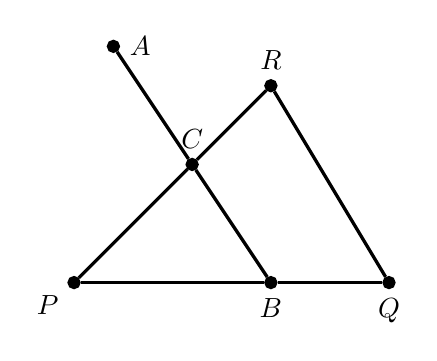
\begin{tikzpicture}
    \tikzstyle{point}=[circle,thick,draw=black,fill=black,inner sep=0pt,minimum width=4pt,minimum height=4pt]
    \node (P)[point,label={[label distance=0cm]210:$P$}] at (0,0) {};
    \node (B)[point,label={[label distance=0cm]-90:$B$}] at (2.5,0) {};
    \node (Q)[point,label={[label distance=0cm]-90:$Q$}] at (4,0) {};
    \node (C)[point,label={[label distance=0cm]90:$C$}] at (1.5,1.5) {};
    \node (R)[point,label={[label distance=0cm]90:$R$}] at (2.5,2.5) {};

    \node (A)[point,label={[label distance=0cm]0:$A$}] at (0.5,3) {};

    \draw[very thick] (P) edge node  {} (B);
    \draw[very thick] (B) edge node  {} (Q);
    \draw[very thick] (P) edge node  {} (C);
    \draw[very thick] (C) edge node  {} (R);

    \draw[very thick] (B) edge node  {} (C);
    \draw[very thick] (C) edge node  {} (A);

    \draw[very thick] (Q) edge node  {} (R);
\end{tikzpicture}
